\documentclass[11pt]{beamer}
\usetheme{Boadilla}
%\usecolortheme[RGB={255, 102, 0}]{structure}
\usepackage[utf8]{inputenc}
\usepackage[francais]{babel}
\usepackage[T1]{fontenc}
\usepackage{amsmath}
\usepackage{amsfonts}
\usepackage{amssymb}
\usepackage[underline=true,rounded corners=false]{pgf-umlsd}
\author{Abdelaziz Khaled}
\title{Production de scénarios d'attaque par model checking UPPAAL}
\date{2 mai 2017} 
%\subject{} 
\begin{document}

\begin{frame}
\titlepage
\end{frame}

%\begin{frame}
%\tableofcontents
%\end{frame}
%%%%%%%%%%%%%%%%%%%%%%% Problème%%%%%%%%%%%%%%%%%%%%%%%%%%%%%%%%%%%%%%%%%%%%%%%%%%
\section{Problèmatique}
\begin{frame}{Problèmatique}
\textcolor{red}{Problème : } générer les scénarios d'attaque à la main est fastidieux, source d'erreurs, et un peu pratique pour les grands systèmes.
\medskip \medskip
\pause
\medskip

\textcolor{red}{But : } développer un Framework qui permet de générer automatiquement les scénarios d'attaque à partir des différentes configurations et différents modèles d'attaquant.
\end{frame}

%%%%%%%%%%%%%%%%%%%%%%%%% section UPPAAl %%%%%%%%%%%%%%%%%%%%%%%%%%%%%%%%%%%%%%%%%%%
\section{UPPAAL}
\subsection{Model checker UPPAAl}
\begin{frame}{Model checker UPPAAl}
\begin{center}
\begin{figure}
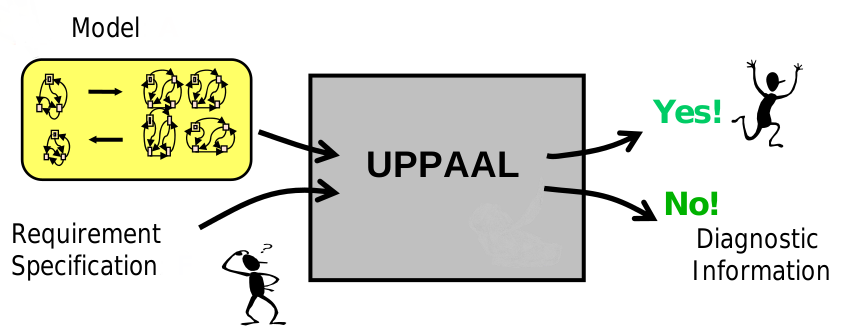
\includegraphics[scale=0.4]{img/mc.png}
%\caption{un schéma représente l'approche de model checking.} 
\end{figure}
\end{center}
\end{frame}

%--------------------------------------------------------------------------
\subsection{Modélisation}

\begin{frame}{Modélisation}
\begin{center}
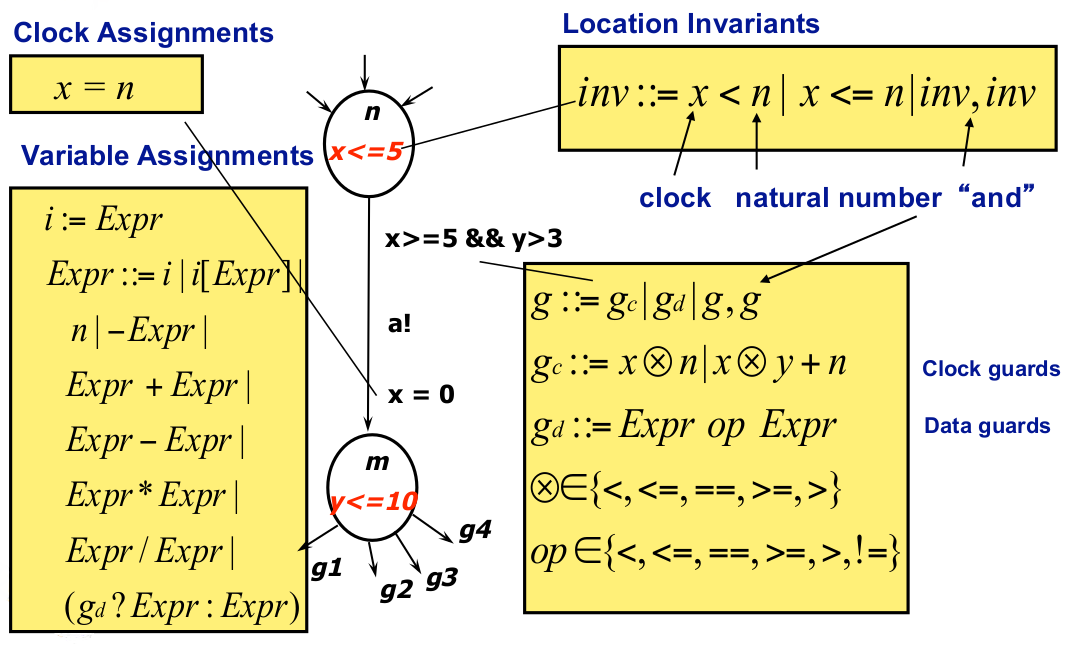
\includegraphics[scale=0.3]{img/model.png} 
\end{center}
\end{frame}
%---------------------------------------------------------------------------
\subsection{Spécification}
\begin{frame}{Spécification}
\begin{itemize}
\item A[]p, A<>p, E<>p, E[]p, p 1 --> p 2
\item Syntaxe :
\end{itemize}
\begin{center}
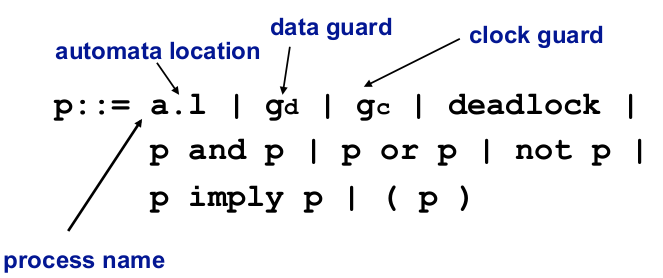
\includegraphics[scale=0.3]{img/phi.png} 
\end{center}
\end{frame}


\subsection{Pourquoi Model checker ?}
\begin{frame}{Pourquoi Model checker ?}
\begin{itemize}
\item Le processus de vérification est automatique et rapide.
\item Les logiques temporelles peuvent facilement exprimer les propriétés.
\item Gère les propriétés de sécurité et de vivacité.
\item Si la spécification n'est pas satisfaite, le model checker produira un \textcolor{red}{contre-exemple}.
\end{itemize}
\end{frame}
\begin{frame}{Contre-exemple = Attaque}
\begin{center}
\huge \textcolor{red}{$\phi \equiv$ AG p}
\end{center}
\medskip

\pause
Un Contre-exemple = Violation de $\phi$\medskip

\pause
\quad\quad\quad\quad\quad\quad\quad\quad\:= Chemin par lequel l'attaquant réussit\medskip

\pause				  
\quad\quad\quad\quad\quad\quad\quad\quad\:= Attaque	

\end{frame}


\subsection{Conception}
\begin{frame}{Conception}
\vspace{-30pt}
\begin{center}
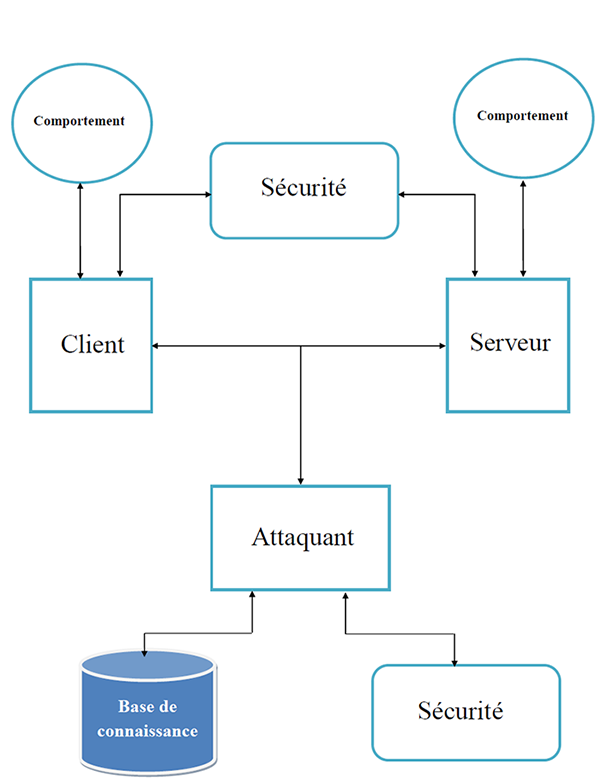
\includegraphics[scale=0.3]{img/conception.png} 
\end{center}
\end{frame}

%%%%%%%%%%%%%%%%%%%%%%% Etude de cas%%%%%%%%%%%%%%%%%%%%%%%%%%%%%%%%%%%%%%%%%%%%%%%%%%
\section{Étude de cas}
\begin{frame}{Étude de cas}
\begin{columns}
	   \begin{column}{0.5\textwidth}
		\vspace{-30pt}
			\begin{figure}[H]
				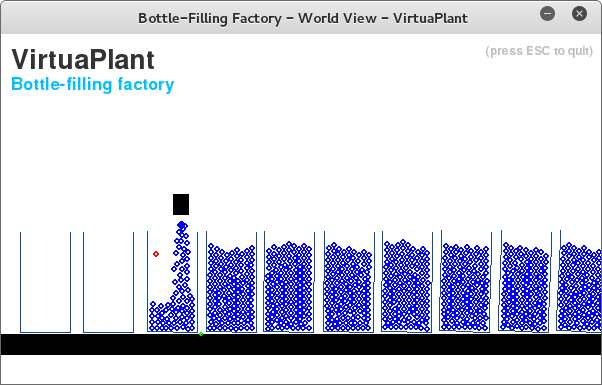
\includegraphics[scale=0.3]{img/virtualPlant.png} 
			\end{figure}
		\end{column}
		\begin{column}{0.5\textwidth}
			\vspace{-30pt}			
			\begin{itemize}
				\item Un tapis roulant. 
				\item Un capteur détecte la position des bouteilles.
				\item Une Valve.
				\item Un autre capteur permet de détecter lorsque la bouteille est pleine.
			\end{itemize}
		\end{column}
		
	\end{columns}
\vspace{20pt}
\pause
Propriétés à préserver  :
\begin{enumerate}
\item Forcer l'ouverture de la valve quel que soit l'état des capteurs.	
\item Forcer le tapis roulant à avancer quel que soit l'état des capteurs.
\item Forcer l'ouverture de la valve et le tapis roulant à avancer quel que soit l'état des capteurs.
\end{enumerate}
\end{frame}
\subsection{Configuration 1}
\begin{frame}{Configuration 1}
\begin{center}
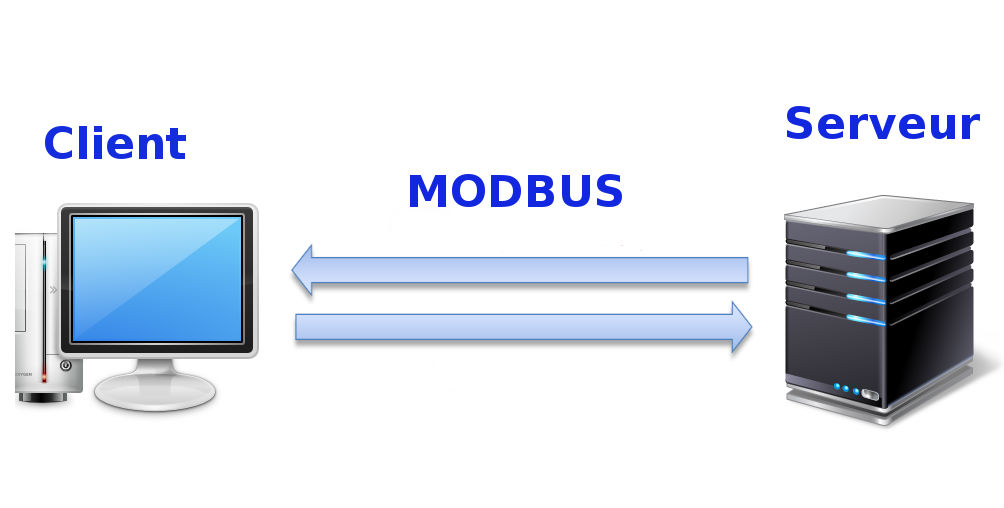
\includegraphics[scale=0.2]{img/conf1.jpg} 
\end{center}
\medskip
\pause
\textbf{Résultat :}\newline

Dans cette configuration toutes les propriétés sont violées.
\medskip
\end{frame}

\begin{frame}{Configuration 1}
%%%%%%%%%%%%% Scénario 1%%%%%%%%%%%%%%%%%%%%%%%%%%
\fontsize{3}{2}\selectfont
\begin{center}
\begin{figure}
\begin{sequencediagram}
  \tikzstyle{inststyle}+=[{font=\tiny}]
  \def\unitfactor{.6}

  \newinst{instance 1}
  {Client}

  \newinst[3cm]{instance 2}
  {Attaquant}

  \newinst[3cm]{instance 3}
  {Serveur}

  \tikzstyle{instcolordienst}=[fill=black!25]
  \tikzstyle{instcolorbuerger}=[fill=black!25]
    
   	  
  \messcall{instance 1}{écrire(run:=true)}{instance 3}
  \messcall{instance 3}{OK}{instance 1}
  \messcall{instance 1}{lire(motor)}{instance 2}
  \textcolor{red}{\messcall{instance 2}{écrire(nozzle:=true)}{instance 3}}
 
\end{sequencediagram}
\vspace{30pt}
\caption{Un exemple de scénario pour l'attaque 1.}
\end{figure}
\end{center}

\end{frame}

\begin{frame}{Configuration 1}
%%%%%%%%%%%%% Scénario 1%%%%%%%%%%%%%%%%%%%%%%%%%%
\fontsize{3}{2}\selectfont
\begin{center}
\begin{figure}
\begin{sequencediagram}
  \tikzstyle{inststyle}+=[{font=\tiny}]
  \def\unitfactor{.6}

  \newinst{instance 1}
  {Client}

  \newinst[3cm]{instance 3}
  {Serveur}
  
  \newinst[3cm]{instance 2}
  {Attaquant}


  \tikzstyle{instcolordienst}=[fill=black!25]
  \tikzstyle{instcolorbuerger}=[fill=black!25]

  \messcall{instance 1}{écrire(run:=true)}{instance 3}
  \messcall{instance 3}{OK}{instance 1}
  \textcolor{red}{\messcall{instance 2}{écrire(nozzle:=true)}{instance 3}}
 
\end{sequencediagram}
\vspace{30pt}
\caption{Un deuxième exemple de scénario pour l'attaque 1.}

\end{figure}
\end{center}

\end{frame}

\subsection{Configuration 2}
\begin{frame}{Configuration 2}
\begin{center}
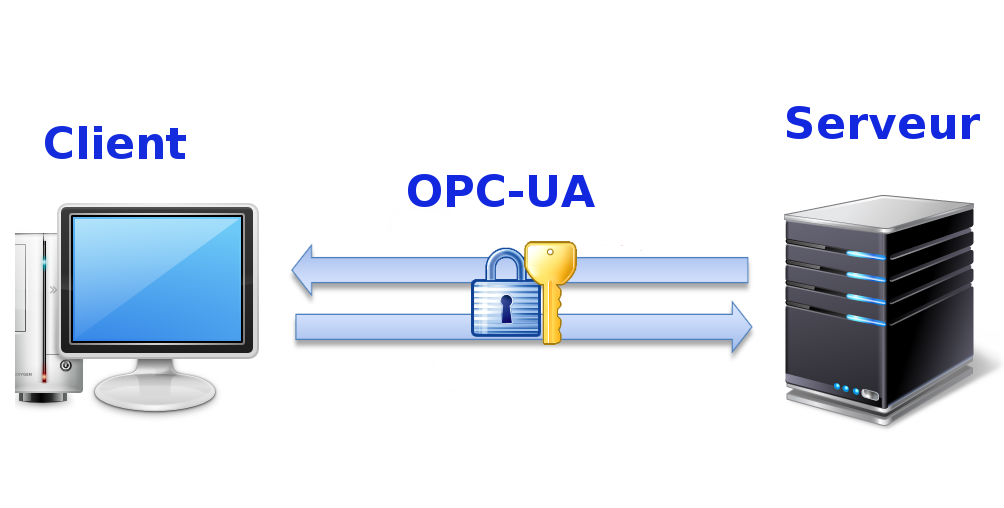
\includegraphics[scale=0.2]{img/conf2.jpg} 
\end{center}
\medskip
\pause
\textbf{Résultat :}\newline

Dans cette configuration aucune attaque trouvée.
\medskip

\end{frame}

\subsection{Configuration 3}
\begin{frame}{Configuration 3}
\begin{center}
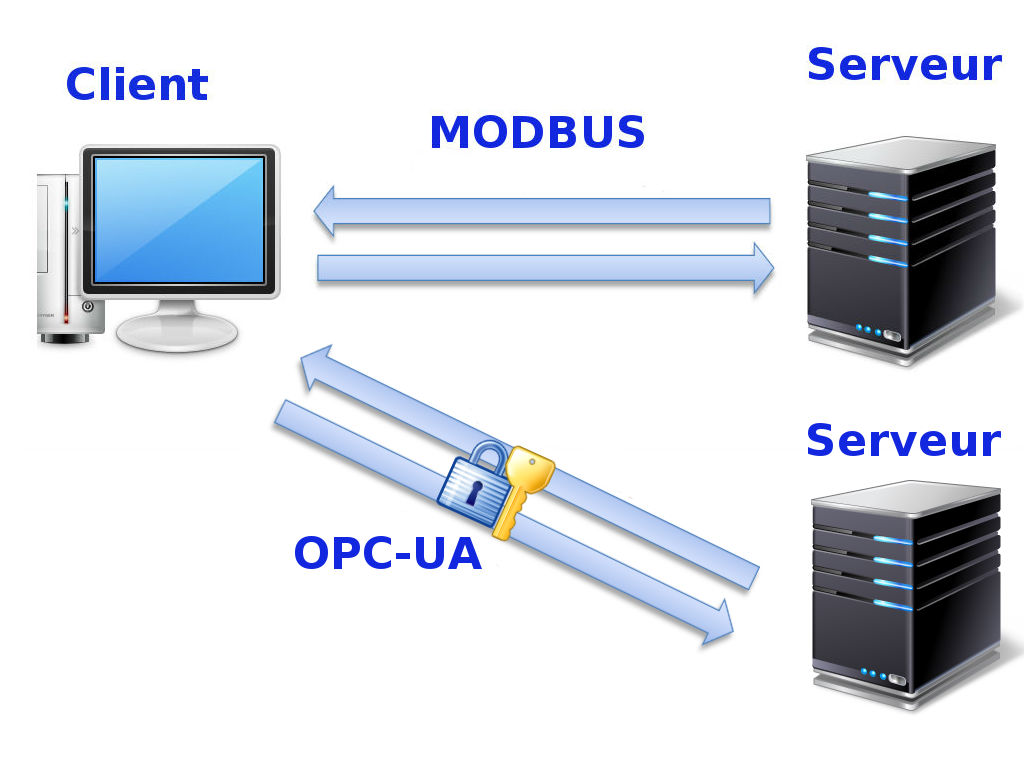
\includegraphics[scale=0.2]{img/conf3.jpg} 
\end{center}
\end{frame}

\begin{frame}{Configuration 3}
\textbf{Serveur MODBUS :}
\begin{itemize}
\item Un tapis roulant.
\item Un capteur détecte la position des bouteilles.\newline
\end{itemize}

\textbf{Serveur OPC-UA :}
\begin{itemize}
\item Une valve.
\item Un capteur permet de détecter lorsque la bouteille est pleine.
\end{itemize}

\medskip
\pause
\textbf{Résultat :}\newline

Dans cette configuration toutes les propriétés sont violées.
\medskip

\end{frame}

\begin{frame}{Configuration 3}
%%%%%%%%%%%%% Scénario 1%%%%%%%%%%%%%%%%%%%%%%%%%%
\fontsize{3}{2}\selectfont
\begin{center}
\begin{figure}
\begin{sequencediagram}
  \tikzstyle{inststyle}+=[{font=\tiny}]
  \def\unitfactor{.6}

  \newinst{instance 1}
  {Client}

  \newinst[1cm]{instance 2}
  {Attaquant}

  \newinst[1cm]{instance 3}
  {OPC-UA}
  
  \newinst[1cm]{instance 4}
  {MODBUS}

  \tikzstyle{instcolordienst}=[fill=black!25]
  \tikzstyle{instcolorbuerger}=[fill=black!25]

  \messcall{instance 1}{écrire(run:=1)}{instance 3}
  \messcall{instance 3}{OK}{instance 1}
  \messcall{instance 1}{lire(motor)}{instance 2}
  \textcolor{red}{\messcall{instance 2}{écrire(bottle:=true)}{instance 4}}
\end{sequencediagram}
\vspace{30pt}
\caption{Un exemple de scénario pour l'attaque 1.}
\end{figure}
\end{center}
\end{frame}
\begin{frame}{Suite}
\begin{itemize}
\item Faire des expérimentations avec des grands exemples pour savoir les limites de :
\begin{itemize}
\item notre modèle.
\item modèle checker.
\end{itemize}
%\item
\item La comparaison avec des approches de vérification de protocoles cryptographiques.
\end{itemize}
\end{frame}
\begin{frame}
\begin{center}
{\huge \textbf{\textit{Merci pour votre\\ attention}}}
\end{center}
\end{frame}
\end{document}

